%%==================================================================%%
%% Author : Sa�udo Olmedo, Ignacio                                  %%
%% Author : S�nchez Barreiro, Pablo                                 %%
%% Version: 1.1, 21/04/2014                                         %%
%%                                                                  %%
%% Memoria del Proyecto Fin de Carrera                              %%
%% M2M, Archivo ra�z                                                %%
%%==================================================================%%

\chapterheader{Model to text}{Model to text}
\label{chap:domain}

Este cap�tulo describe el primer paso del proceso de transformaci�n de acuerdo al proceso de desarrollo dirigido por modelos. El principal objetivo de esta fase es la transformaci�n de un modelo definido en UML  a un modelo en Cassandra. La primera fase consiste en la definici�n de un metamodelo que defina el modelado en Cassandra. En segundo lugar debemos  definir las reglas de transformaci�n para convertir un modelo UML a un modelo en Cassandra utilizando para ello el lenguaje ETL.

\chaptertoc

\section{Introducci�n}
\label{domain:sec:intro}
%%==================================================================%%
%% Author : Sa�udo Olmedo, Ignacio                                  %%
%% Author : S�nchez Barreiro, Pablo                                 %%
%% Version: 1.4, 21/06/2014                                         %%
%%                                                                  %%
%% Memoria del Proyecto Fin de Carrera                              %%
%% M2M/Introduccion                                                 %%
%%==================================================================%%


El primer paso a la hora de desarrollar un generador de c�digo es establecer una serie de reglas de correspondencia entre el modelo de entrada y el modelo de salida. Estas reglas han de contemplar los distintos tipos de elementos que pueden aparecer en ambos lenguajes, as� como elementos que no aparecen en uno de los dos lenguajes y tiene importancia en el otro.
En este caso, consiste en establecer reglas de correspondencia entre elementos UML 2.0 y el lenguaje Cassandra Query Language (CQL).
Para la definici�n de estas reglas se ha utilizado el lenguaje Epsilon Transformation Language (ETL) y el lenguaje Epsilon Object Language (EOL).
Tras implementar estas reglas y comprobar que son funcionales se puede implementar el generador de c�digo pero este tema se trata en el siguiente capitulo.
En cuanto a la construcci�n EMF
El meta-modelo utilizado de UML es el que proporciona la herramienta EMF por defecto.

\section{Metamodelo Cassandra}
\label{domain:sec:metamodelo}
%%==========================================================================%%
%% Author : Sa�udo Olmedo, Ignacio                                          %%
%% Author : S�nchez Barreiro, Pablo                                         %%
%% Version: 1.2, 23/04/2014                                                 %%
%%                                                                          %%
%% Memoria del Proyecto Fin de Carrera                                      %%
%% M2M/MetamodeloCassandra                                                  %%
%%==========================================================================%%
Como hab�amos descrito en el capitulo anterior la base del proceso de transformaci�n entre modelos
parte del metamodelo. El metamodelo utilizado de UML en este proyecto es el que nos proporciona Epsilon, dicho metamodelo sigue el est�ndar de UML 2.0. Sin embargo nos hace falta un metamodelo que defina el lenguaje de Cassandra. Dicho metamodelo fue proporcionado por Pablo S�nchez Barreiro. El metamodelo sufri� algunos cambios respecto al inicial debido a exigencias del proyecto. El metamodelo de Cassandra es el que se ve en la figura Figura~\ref{back:fig:metamodeloCassandra}.

\begin{figure}[!tb]
  \centering
  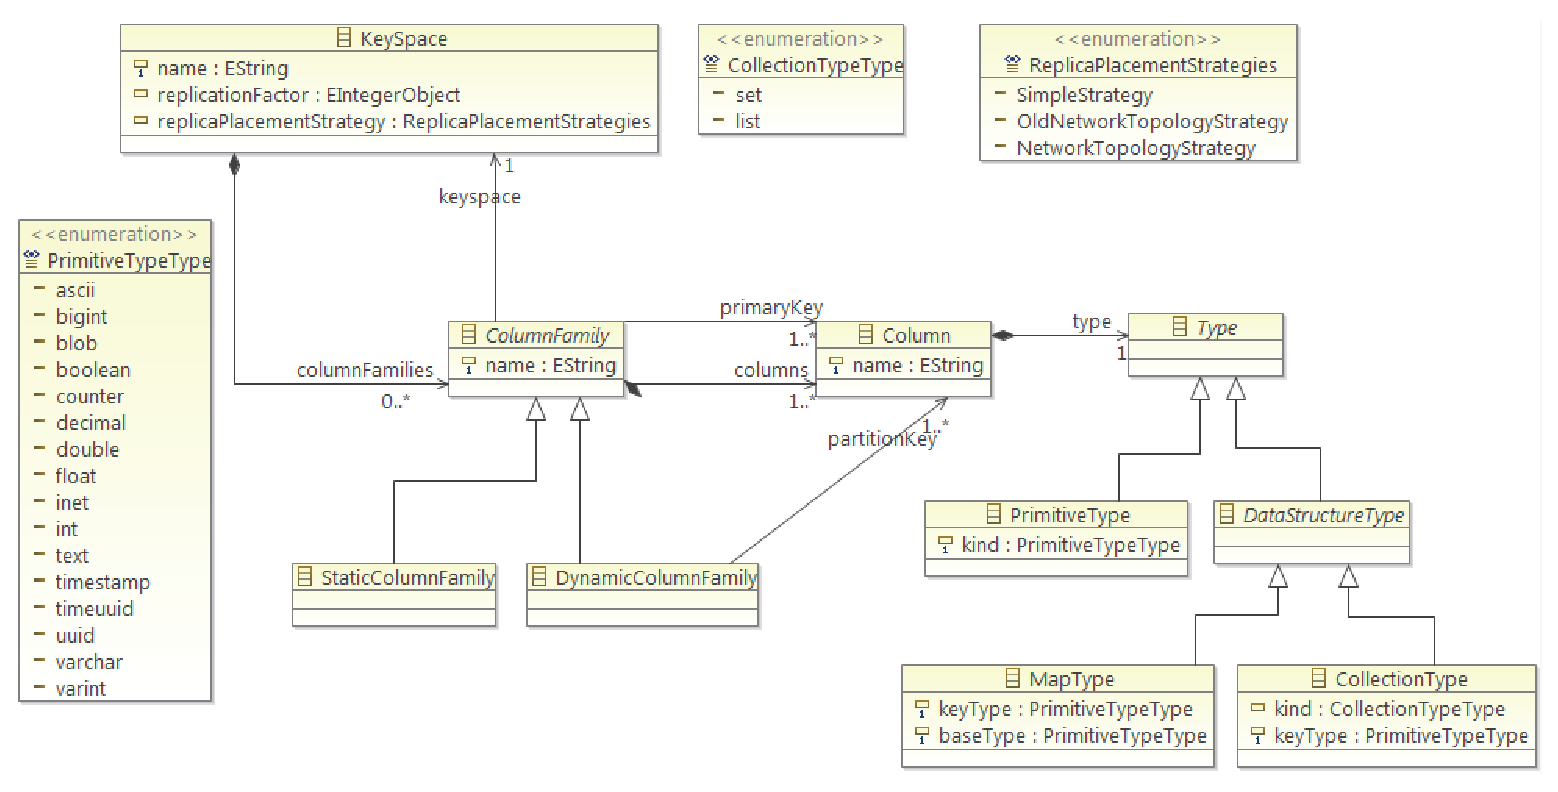
\includegraphics[width=.8\linewidth]{m2m/images/ecoreDiag.eps} \\
  \caption{Metamodelo Cassandra}
  \label{back:fig:metamodeloCassandra}
\end{figure} 

El eje central del metamodelo es el KeySpace, el KeySpace es el equivalente a la base de datos en el modelo relacional, la clase del metamodelo KeySpace cuenta con los atributos: nombre utilizado para denominar el KeySpace, [cassandra] replicationFactor n�mero de servidores de Cassandra de los que se debe guardar un registro u obtener una respuesta al recuperar alg�n registro y replicaPlacementStrategy que es la estrategia de replicaci�n que se va a tomar, estrategias tenemos tres tipos: %[http://www.datastax.com/docs/1.0/cluster_architecture/replication]:
SimpleStrategy: Esta estrategia es la estrategia de replicaci�n utilizada por defecto al crear un KeySpace utilizando Cassandra. Es utilizada para cl�steres de data centers simples.
NetworkTopologyStrategy: Utilizada cuando se tiene (o se va a tener) el cl�ster desplegado a trav�s de m�ltiples data centers. Esta estrategia especifica cu�ntas r�plicas se desean en cada data center.
OldNetworkTopologyStrategy: Se utiliza para proporcionar retro compatibilidad con instalaciones Cassandra antiguas.

A continuaci�n tenemos la clase ColumnFamily equivalente a las tablas en el modelo relacional, dentro de las CF encontramos dos tipos: las StaticColumnFamily y las DynamicColumnFamily. Recordamos que la CF est�tica es el equivalente a la tabla en el modelo relacional, sin embargo la CF din�mica es utilizada para la recuperaci�n de datos eficiente, algo similar a las vistas del modelo relacional. %[http://www.datastax.com/docs/1.1/ddl/column_family#dynamic-column-families]. 
En CQL el orden de definici�n de las claves importa, en la primera columna se define la Partition Key esta tiene la propiedad de que todas las filas que comparten la misma Partition Key se almacenan en el mismo nodo f�sico %[http://www.datastax.com/docs/1.1/ddl/indexes].
Adem�s, la inserci�n, actualizaci�n o eliminaci�n de filas que comparten la Partition Key para una CF determinada se realizan de forma at�mica. Es posible tener una Partition Key compuesta, es decir, una Partition Key formada por varias columnas, en CQL esto se define utilizando par�ntesis para delimitar el conjunto de partici�n.
Dentro de las ColumnFamily encontramos Columns estos son los valores que se almacenan en las Column Families las cuales tienen el nombre como atributo y un tipo de dato. Dentro de los tipos encontramos dos clases, PrimitiveType y DataStructureType, el primero define los tipos primitivos, por ejemplo entero, texto, uuid, etc..
DataStructureType define las colecciones, estas pueden ser de dos tipos MapType o bien CollectionType, ambas  tiene un atributo llamado KeyType para definir el tipo primitivo que las caracteriza. MapType cuenta con un atributo llamado baseType de tipo primitivo que define el segundo tipo de dato del mapa. Dentro de CollectionType encontramos un atributo llamado kind que define el tipo de colecci�n que vamos a utilizar esta puede ser o bien tipo set o tipo list. M�s adelante se explica que caracter�sticas re�ne cada colecci�n y mapa y cuando se utilizan.


\section{Transformaci�n de Modelo UML a Cassandra}
\label{domain:sec:transformation}
%%==================================================================%%
%% Author : Sa�udo Olmedo, Ignacio                                  %%
%% Author : S�nchez Barreiro, Pablo                                 %%
%% Version: 1.4, 29/04/2014                                         %%
%%                                                                  %%
%% Memoria del Proyecto Fin de Carrera                              %%
%% M2M/Reglas Transformaci�n UML a Cassandra                        %%
%%==================================================================%%

Una vez definido el metamodelo de Cassandra utilizamos ETL para establecer las reglas de transformaci�n entre UML y Cassandra CQL. Recordamos que el lenguaje ETL es el lenguaje que utiliza Epsilon para la transformaci�n entre modelos basado en reglas. A continuaci�n se presenta una explicaci�n de las reglas junto con el c�digo correspondiente.
Las reglas de transformaci�n son definidas en [docPablo]. A continuaci�n se detalla c�mo se han implementado dichas reglas en el lenguaje de definici�n de reglas de transformaci�n ETL.
Como vemos estas dos reglas transforman una clase definida en UML a una Column Family est�tica de Cassandra (el equivalente a una tabla en el sistema de bases de datos relacionales).
L a primera regla es definida para las clases que tengan un atributo clave definido, para ello se utiliza la propiedad "isID" la cual define que ese atributo identifica a la clase de forma �nica.  La segunda para las clases sin atributo clave definido. El proceso de transformaci�n es similar en ambas reglas, en primer lugar se asigna la Column Family al KeySpace que le corresponde, se copia el nombre de la clase a la Column Family y se a�ade al conjunto de Column Families del KeySpace. Sin embargo en la segunda regla se crea un atributo que va a ser la clave de esa Column Family ya que no tiene, dicha clave tendr� de nombre el nombre de la clase el distintivo "\_ID" y ser� de tipo uuid.
Dichas reglas est�n definidas en el punto 5.3 del documento.
La siguiente regla define como se realiza la transformaci�n de un atributo del modelo UML a una columna del modelo Cassandra. Para ello en primer lugar se define una guarda para que la transformaci�n se haga solo de los atributos de clase y no los atributos de relaci�n. A continuaci�n se realiza un filtro para evitar la adici�n de columnas que no pertenezcan al modelo de datos. Una vez hecho esto hay que diferenciar dos tipos de atributos, aquellos cuya tama�o sea igual a 1 y aquellos cuyo tama�o sea mayor de 1. En cuanto a los atributos de tama�o igual a 1 se realiza la transformaci�n del atributo copiando su tipo de dato. Respecto a los atributos de tama�o mayor de 1 se aplica la siguiente regla: Aquellos atributos que sean �nicos y no ordenados son definidos como tipo "set" de Cassandra. En caso contrario se definen como tipo list.
A continuaci�n en ambos casos se realiza la transformaci�n correspondiente del tipo de dato UML a Cassandra se copia el nombre y se a�ade la columna ya transformada a la Column Family correspondiente.
Finalmente en caso de que el atributo sea clave de la clase se a�ade a la Column Family como Primary Key. El c�digo correspondiente a esta regla es el siguiente figura~\ref{back:code:reglaTrans}

\begin{figure}[!tb]
\begin{center}
\begin{footnotesize}
\begin{verbatim}
--------------------------------------------------------
//5.5 Attribute with primitive type transformation
rule Attribute2Column
transform attribute : UML!Property
to column : nosql!Column {
    guard: ((""+attribute.qualifiedName).contains("Data::") and attribute.type.isKindOf(UML!PrimitiveType))

    //filtramos para evitar a�adir columnas ajenas al modelo de datos
    for(cfamily in kspace.columnFamilies){	
    
        if(attribute.qualifiedName=="Data::"+cfamily.name+"::"+attribute.name){
        
            //5.5 Attribute with primitive type transformation->Attributes with upper bound = 1
            if(attribute.upper=1){
                //transformacion del atributo en una columna basica
                var type : new nosql!PrimitiveType;
                type.kind=umlType2modelType(attribute.type.name);
                column.type=type;
            }
            //5.5 Attribute with primitive type transformation->Attributes with upper bound > 1
            else if(attribute.upper<>0){
                //transformacion del atributo en un set o list
                var ctype : new nosql!CollectionType;

                if(attribute.isUnique and not attribute.isOrdered)//set
                    ctype.kind=nosql!CollectionTypeType#set;
                else//list
                    ctype.kind=nosql!CollectionTypeType#list;

                ctype.keyType=umlType2modelType(attribute.type.name);
                column.type=ctype;
            }
            
            column.name=attribute.name;			
            cfamily.columns.add(column);		

            //5.1 Assignment of keys to classes
            if(attribute.isID)
                cfamily.primaryKey.add(column);
                
        }
    }
}
--------------------------------------------------------
\end{verbatim}
\end{footnotesize}
\end{center}
\caption{Regla de transformaci�n XX}
\label{back:code:reglaTrans}
\end{figure}

La siguiente regla define como se realiza la transformaci�n de los atributos de las asociaciones entre clases UML.
En primer lugar hay que diferenciar como se tratan las asociaciones, aquellas asociaciones cuyo extremo tenga una cardinalidad igual a uno y aquellas con una cardinalidad mayor de uno.
Para los extremos con cardinalidad igual a uno se crea una columna que ser� a�adida en la Column Family del otro extremo de la relaci�n, esta columna nueva es una copia de la Primary Key de la Column Family fuente, el nombre de la nueva columna es la composici�n del nombre de la Column Family y del nombre de la Primary Key, el tipo de la nueva columna es el mismo del de la Primary Key de la Column Family fuente. Esto se comprende mejor con el ejemplo propuesto m�s adelante.

Para los extremos con cardinalidad mayor de uno, se crea una Column Family din�mica. En la primera columna se define la Partition Key. El resto de columnas de la Primary Key se utilizan para definir las llamadas Clustering Columns, estas se utilizan para la recuperaci�n de filas de manera eficiente.
La transformaci�n utilizada para este tipo de Column Family es la siguiente: Esta CF din�mica est� compuesta de dos columnas, la primera columna y segunda columna juegan el papel de Partition Key de la CF, la primera columna se construye de la misma manera que el caso anterior, se copia el nombre y el tipo de la Primary Key del extremo de la asociaci�n fuente. La segunda columna de la misma manera toma los datos (nombre y tipo de la PK) del otro extremo de la asociaci�n. El rol de Cluster Key lo desempe�a la primera columna creada.
El nombre de la CF ser� la concatenaci�n del nombre de las CF de ambos extremos (primero fuente, segundo extremo fin de la asociaci�n).
En resumen la definici�n de la Primary Key es la siguiente:
\begin{enumerate}
\item Partition Key: Primera columna  (fuente de la asociaci�n), segunda columna (extremo de la asociaci�n).
\item Clustering Columns: Primera columna (fuente de la asociaci�n).
\end{enumerate}
	

En cuanto a la transformaci�n de variables de tipo primitivo se define la siguiente operaci�n de esta manera podemos convertir un tipo primitivo UML a su equivalente en Cassandra. Dicha regla est� definida en el punto 5.4 del documento.
Como se explicaba en el anterior capitulo �l para ello nos har� falta realizar la creaci�n de un modelo UML  de acuerdo a las principales reglas de este lenguaje de modelado.
En primer lugar se ha utilizado la herramienta EMF descrita anteriormente para la creaci�n del modelo, a continuaci�n se ha exportado este modelo UML a la herramienta de transformaci�n de modelos Epsilon.


\section{Caso de estudio}
\label{domain:sec:casoEstudio}
%%==================================================================%%
%% Author : Sa�udo Olmedo, Ignacio                                  %%
%%          S�nchez Barreiro, Pablo                                 %%
%% Version: 1.2, 18/06/2014                                         %%
%%                                                                  %%
%% Memoria del Proyecto Fin de Carrera                              %%
%% Planificacion/CasoEstudio                                        %%
%%==================================================================%%

\begin{figure}[!tb]
  \centering
  \includegraphics[width=.8\linewidth]{m2m/images/twissandra.eps} \\
  \caption{Modelo UML Twissandra}
  \label{back:fig:twissandra}
\end{figure}

Esta secci�n presenta \emph{Twissandra}, el caso de estudio que se utilizar� lo largo de este proyecto. Twissandra es un proyecto creado para aprender como utilizar Cassandra. El modelo UML correspondiente a Twissandra se puede ver en la figura~\ref{back:fig:twissandra}. Twissandra es una versi�n simplificada de Twitter.

Twitter\footnote{} es una red social de microblogging, actualmente est� muy extendida, que permite escribir a sus usuarios peque�os mensajes de texto, denominados \emph{tweets}. Un \emph{tweet} es simplemente un texto con un l�mite de 140 caracteres publicado a una hora determinada. La colecci�n de todos los tweets publicados por un usuario cronol�gicamente ordenados determinan su \emph{userline}.

Cada usuario registrado en Twitter puede seguir a otros usuarios registrados. Cuando decimos, por ejemplo, que Pedro sigue a Mar�a significa que Pedro recibir� en su cuenta todos los mensajes que publique Mar�a. En este caso, se dice que Pedro es un \emph{follower} de Mar�a. De esta forma, cada usuario tiene asociado un \emph{timeline} que no es m�s que la colecci�n de todos los \emph{tweets} publicados por las personas a las que sigue ordenados cronol�gicamente, es decir, por fecha de publicaci�n. 

Los principales casos de uso de \emph{Twissandra} son: 

\begin{enumerate}
    \item Obtener el \emph{timeline} de un usuario determinado. 
    \item Obtener el \emph{userline} de un usuario determinado. 
    \item Obtener la lista de usuarios que un usuario est� siguiendo.  
    \item Obtener la lista de usuarios que est�n siguiendo a un usuario espec�fico. 
\end{enumerate}

Las dos �ltimas listas deben se deben devolver ordenadas cronol�gicamente.

%%========================================================================================%%
%% NOTA(Pablo): Esta justificaci�n es d�bil, as� que mejor quitarla                       %%
%%========================================================================================%%

Como vemos \imp{Twissandra} es una versi�n simplificada de Twitter. Sin embargo, se considera un buen ejemplo a analizar ya que Twitter goza de gran popularidad y es una de las redes sociales m�s usadas del mundo. 

Una vez entendido esto en los siguientes cap�tulos se procede a detallar el proceso de creaci�n de un repositorio de datos en Cassandra que cubra los casos de usos citados anteriormente describiendo los procesos de transformaci�n entre modelos que se realizaran as� como la generaci�n de c�digo del repositorio de datos en Twissandra.


\section{Pruebas}
\label{domain:sec:pruebas}
%%=======================================================================%%
%% Author : Sa�udo Olmedo, Ignacio                                       %%
%% Author : S�nchez Barreiro, Pablo                                      %%                                                                      %%                                                                       %%
%% Version: 2.0, 25/06/2014                                              %%                                                                         %%                                                                       %%
%% Memoria del Proyecto Fin de Carrera                                   %%
%% M2M/Pruebas con EUnit                                                 %%   %%=======================================================================%%

Una vez implementado el generador de c�digo la siguiente tarea consiste en comprobar que el c�digo generado funciona correctamente.
Para ello creamos, una serie de pruebas unitarias que permitan comprobar que el funcionamiento de los generadores de c�digo es correcto para un conjunto de modelos de entrada.

Estas pruebas unitarias se han implementado en EUnit, el lenguaje de definici�n de pruebas de la suite Epsilon. EUnit funciona de una manera muy similar a JUnit, pero aplicado a los lenguajes de la suite Epsilon, como EGL. Utilizamos EUnit para comprobar que el funcionamiento del generador de c�digo es correcto, para ello se dise�an una serie de casos de prueba y se crea la salida esperada de cada uno de esos casos de prueba de forma manual.
A continuaci�n, se ejecuta el caso de prueba creado en EUnit y se comprueba que la salida generada coincide con la esperada, que es la creada manualmente. Adem�s comprobamos con casos espec�ficos que la cobertura del c�digo es del 100%.

El �nico problema surge por un problema de defecto en la herramienta EUnit, la funci�n de comparaci�n de ficheros llamada assertEqualFiles obliga a que ambos ficheros sean estrictamente iguales por lo que para crear casos de prueba tanto el c�digo de entrada de prueba como el c�digo generado a testear han de ser iguales, espacios y saltos de l�nea incluidos.


\section{Sumario}

Durante este cap�tulo se ha descrito
